%%%%%%%%%%%%%%%%%%%%%%%%%%%%%%%%%%%%%%%%%
% Friggeri Resume/CV
% XeLaTeX Template
% Version 1.0 (5/5/13)
%
% This template has been downloaded from:
% http://www.LaTeXTemplates.com
%
% Original author:
% Adrien Friggeri (adrien@friggeri.net)
% https://github.com/afriggeri/CV
%
% License:
% CC BY-NC-SA 3.0 (http://creativecommons.org/licenses/by-nc-sa/3.0/)
%
% Important notes:
% This template needs to be compiled with XeLaTeX and the bibliography, if used,
% needs to be compiled with biber rather than bibtex.
%
%%%%%%%%%%%%%%%%%%%%%%%%%%%%%%%%%%%%%%%%%

\documentclass[]{friggeri-cv} % Add 'print' as an option into the square bracket to remove colors from this template for printing

\addbibresource{bibliography.bib} % Specify the bibliography file to include publications

\begin{document}

\header{Arnaud}{Bletterer}{Etudiant en Informatique Graphique} % Your name and current job title/field

%----------------------------------------------------------------------------------------
%	SIDEBAR SECTION
%----------------------------------------------------------------------------------------

\begin{aside} % In the aside, each new line forces a line break
\vspace{3.7cm}

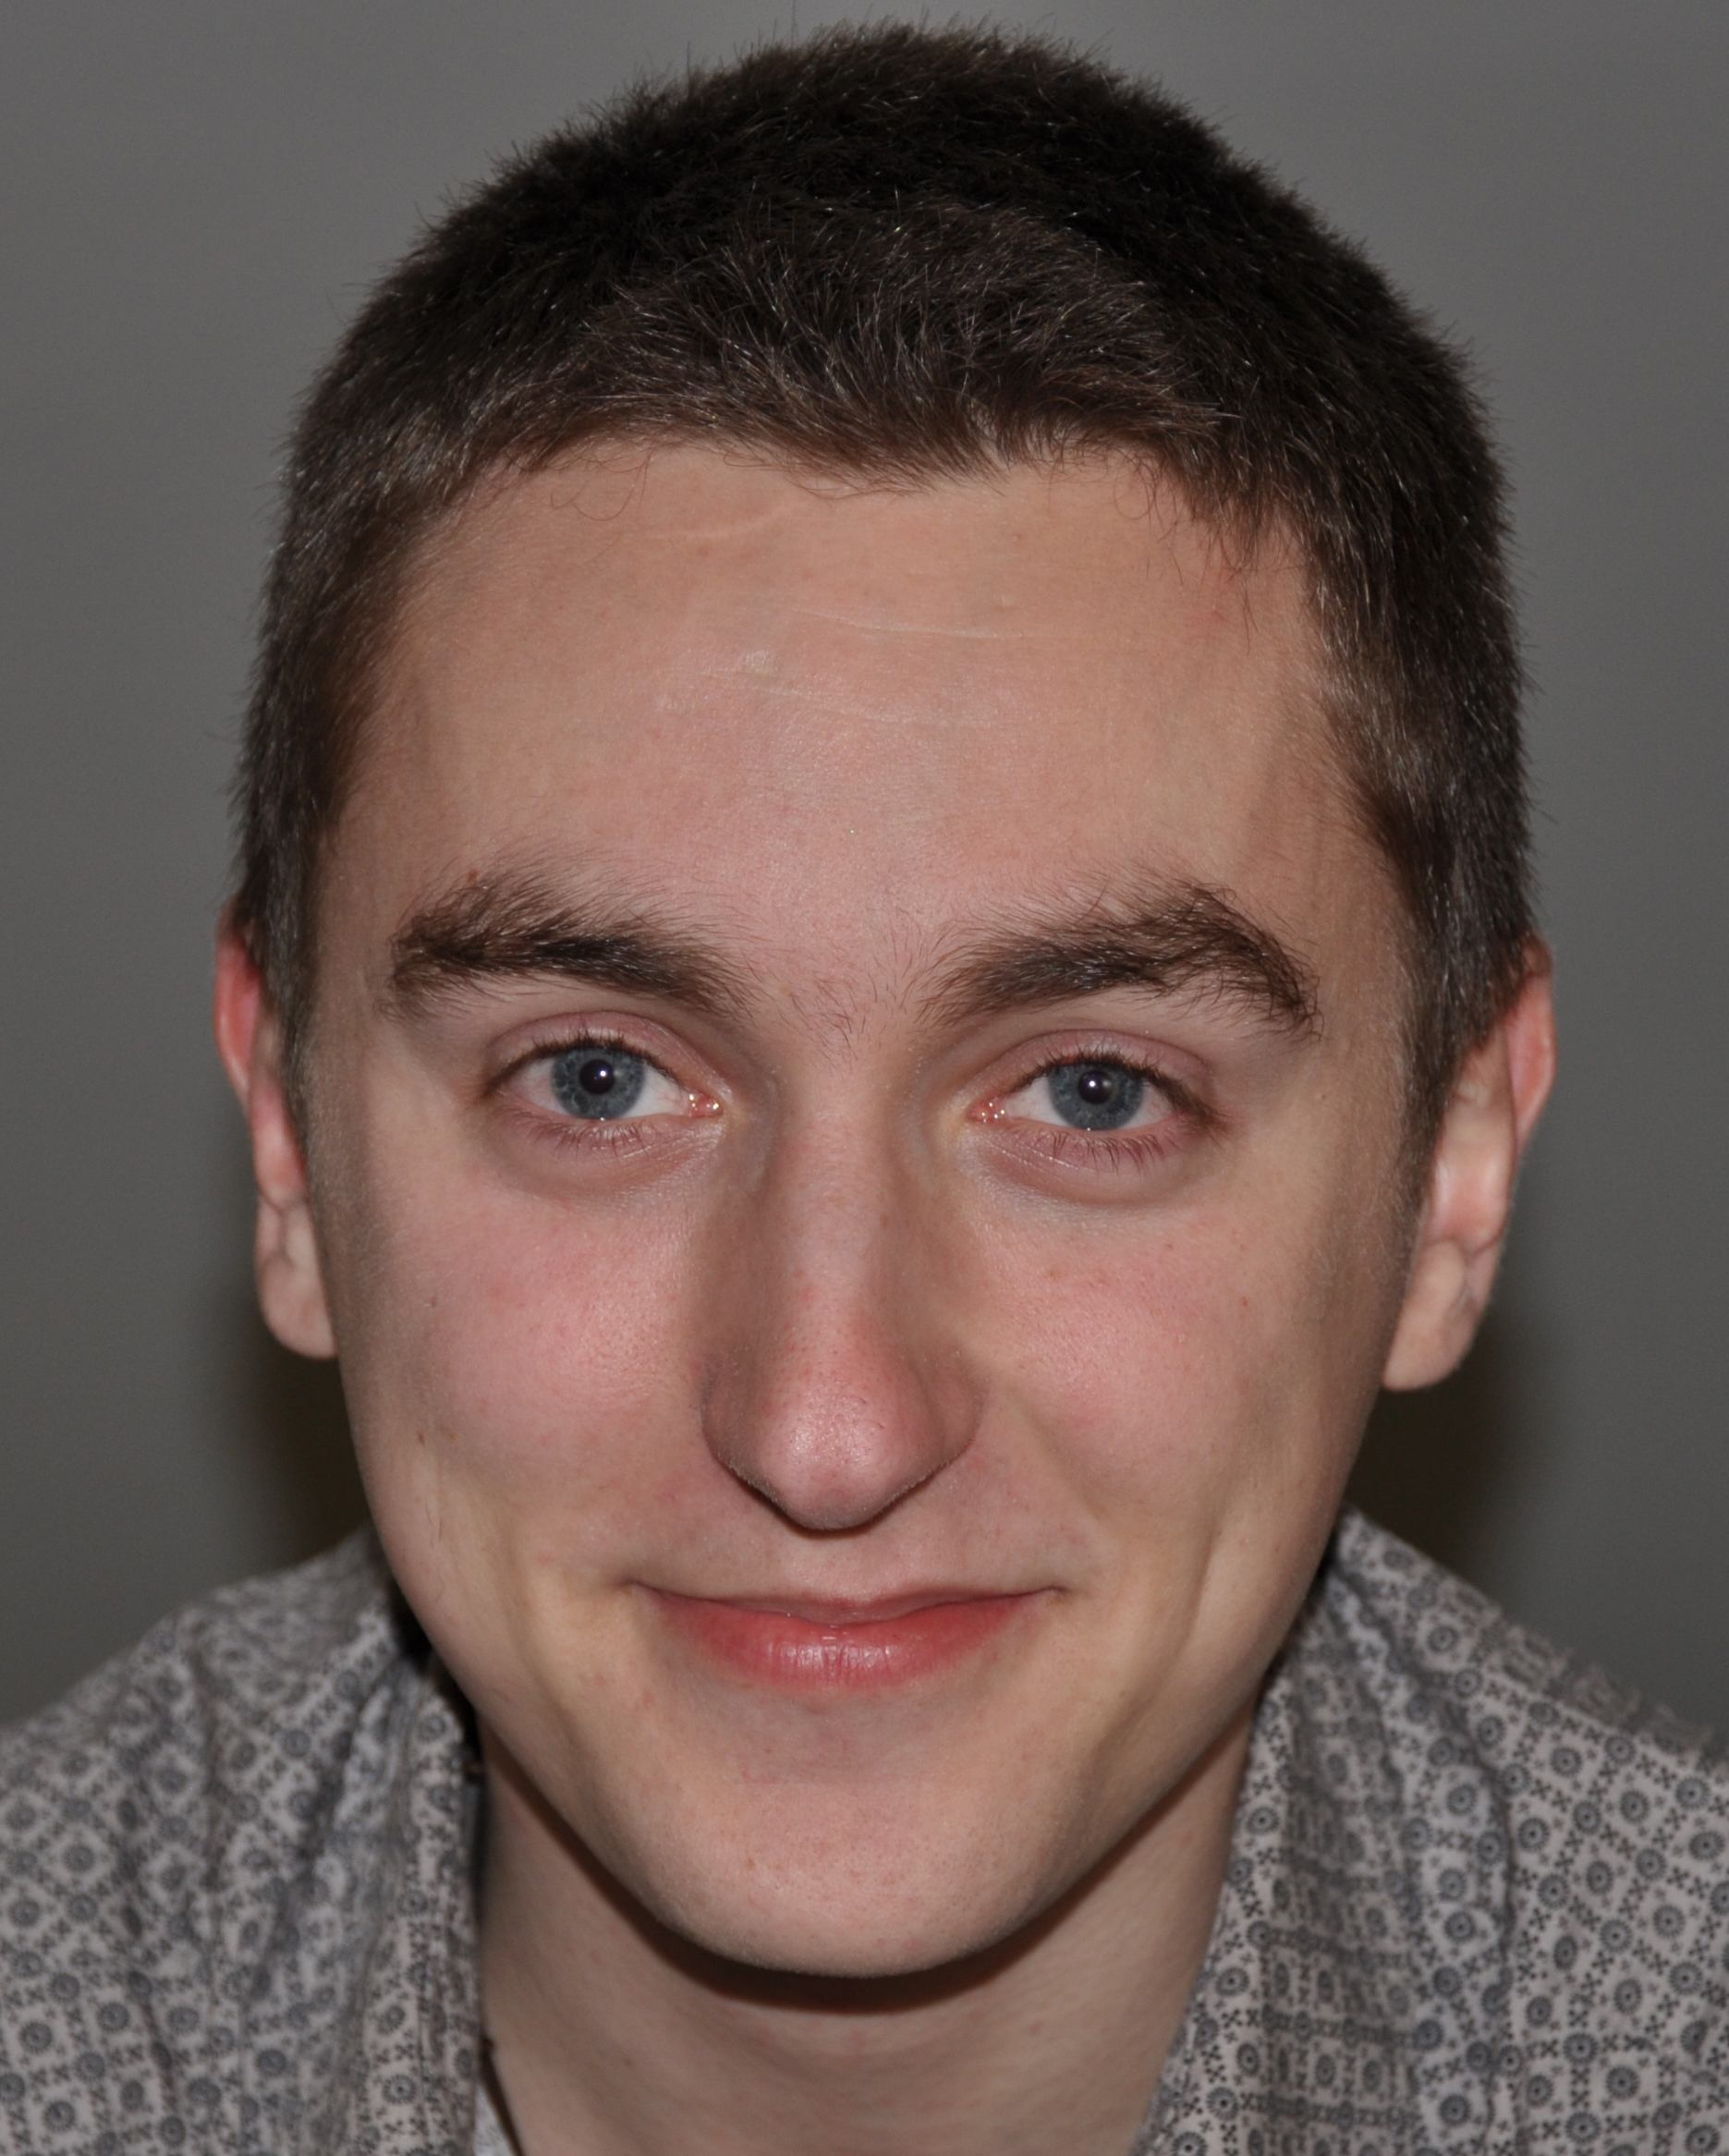
\includegraphics[scale=0.05]{Profil}
\section{Coordonnées}
Arnaud Bletterer
2, Route de Forstheim
67500 Haguenau
FRANCE
~
+333 69 02 09 52
+336 64 32 44 28
~
\href{mailto:arnaud.bletterer@gmail.com}{arnaud.bletterer@gmail.com}
\href{http://abletterer.fr}{http://abletterer.fr}
\section{Langues}
Anglais, avancé
Allemand, scolaire
\end{aside}

%----------------------------------------------------------------------------------------
%	COMMUNICATION SKILLS SECTION
%----------------------------------------------------------------------------------------

\section{Compétences}

%------------------------------------------------
\textbf{Développement Web:}
PHP, HTML5, CSS3, Bootstrap, JavaScript, JQuery

%------------------------------------------------
\textbf{Génie Logiciel:}
C, C++, Java, C\#, SQL, MySQL, Oracle, PL/SQL, T-SQL, Merise, UML

%------------------------------------------------
\textbf{Systèmes:}
Linux, Windows, ShellScript, Systèmes distribués

%------------------------------------------------
\textbf{Synthèse d'Image:}
OpenGL, Cartes combinatoires
%------------------------------------------------

%----------------------------------------------------------------------------------------
%	EDUCATION SECTION
%----------------------------------------------------------------------------------------
\section{Formation}

\begin{entrylist}
%------------------------------------------------
\entry
{2012-2014}
{Master {\normalfont Informatique, Sciences de l'Image}}
{Université de Strasbourg}
{}
%------------------------------------------------
\entry
{2011-2012}
{Licence {\normalfont Informatique}}
{Université de Strasbourg}
{}
%------------------------------------------------
\entry
{2009-2011}
{Diplôme Universitaire de Technologie {\normalfont Informatique}}
{Université de Strasbourg}
{}
%------------------------------------------------
\entry
{2009}
{Baccalauréat {\normalfont Scientifique, Sciences de l'Ingénieur}}
{LEGTI Alphonse Heinrich}
{}
%------------------------------------------------
\end{entrylist}

%----------------------------------------------------------------------------------------
%	WORK EXPERIENCE SECTION
%----------------------------------------------------------------------------------------

\section{Expérience}

\begin{entrylist}
%------------------------------------------------
\entry
{2013--3 mois}
{Projet de développement}
{Université de Strasbourg}
{\emph{Génération de cage et Déformation de l'espace \\ Références : Pierre Kraemer et Dominique Bechmann} \\
Développement d'une application utilisant la librairire CGoGN, développée par le laboratoire ICube, générant une cage selon divers paramètres permettant de déformer un maillage plus ou moins localement.}
%------------------------------------------------
\entry
{2013--3 mois}
{Travail d'étude et de Recherche}
{Université de Strasbourg}
{\emph{Multi-Triangulation\\Références : Lionel Untereiner et Pierre Kraemer} \\
Développement d'une application utilisant la librairire CGoGN, développée par le laboratoire ICube, mettant en place une gestion multi-résolution d'un maillage triangulaire.}
%------------------------------------------------
\entry
{2011--3 mois}
{Stage de fin de DUT}
{REP Solutions Interactive Inc., Québec, Canada}
{\emph{Référence : Alain Marceau} \\
Développeur JavaScript.
\begin{itemize}
\item Etude avancée de la réalisation du café
\item Refonte de l'affichage des résultats de sondages
\item Réalisation de tutoriels pour l'utilisation de l'API Google Analytics
\end{itemize}}
\end{entrylist}

%----------------------------------------------------------------------------------------
%	INTERESTS SECTION
%----------------------------------------------------------------------------------------

\section{Intérêts}

\textbf{Professionnels:} Web design, Cuda, Node.js, Angular.js, RubyOnRails, Dart, Droit de l'Informatique

\textbf{Personnels:} Sport électronique, Athlétisme, Arts Martiaux, Guitare Basse

%----------------------------------------------------------------------------------------

\end{document}